\section{Separating two subgraphs of large list chromatic number}
\label{sec:separability}

We adapt the list-chromatic separability framework of Postle
\cite[Definition~2.4 and Lemmas~2.5--2.6]{Postle2020}.
The next lemma allows the construction to branch. Its proof treats the
alternative in which two disjoint subgraphs cannot both retain nearly all
of the list chromatic number. In that alternative, successive highly
connected regions must overlap substantially. We use these overlaps to
extend a clique model through \(O(\log^4t)\) small districts.
Figure~\ref{fig:separability-round} illustrates one extension.

\begin{lemma}[Separability]
\label{lem:separability}
There is an absolute positive integer \(S\) such that, for all sufficiently
large integers \(t\), every graph \(G\) satisfying
\[
 h(G)<t,\qquad r=\ell(G)\ge 2St
\]
has two vertex-disjoint induced subgraphs \(G_1,G_2\) with
\[
 \ell(G_1),\ell(G_2)\ge r-St.
\]
\end{lemma}

To understand the construction behind the lemma, suppose that no such
pair of subgraphs exists. We carry \(t\) disjoint connected label bags,
each with one tip in a highly connected region of large list chromatic
number. Alongside the bags we keep a \emph{footprint}: the set of all
vertices recorded so far, including unused path vertices. A round adds
adjacencies among a selected group of labels. Inside the current region,
choose two disjoint small districts outside the footprint: one will
supply a rooted clique model on these labels, while the other serves
as a junction. Choose a minimum-total-length system of two paths from
every old tip and every selected model root to distinct junction vertices.

Deleting the accumulated footprint, the districts, and these paths
leaves enough list chromatic number to extract a fresh highly connected
region. The supposition on \(G\) forces the old and fresh regions to
overlap. This overlap makes a second family of \(2t\) paths to the
junction feasible, with distinct freely chosen starts in the fresh
region; again minimize their total length. The two families may
intersect. Lemma~\ref{lem:combine} combines them into disjoint paths
from every old tip and model root, and from \(t\) selected new tips.
Rerouting through the model district installs the clique model;
grouping the path ends in the junction joins each old bag to its new
tip and, for a selected label, to its assigned model bag. Repeating the
construction for suitably chosen groups makes every two label bags
adjacent.

Every district and both original minimizing systems remain in the
footprint. The paths actually extending the bags may have been rerouted
and need not still minimize length; all deletion estimates use the
recorded originals. These paths can have arbitrarily many vertices.
The next lemma bounds the list-coloring cost of the whole footprint.
By Lemma~\ref{lem:additive-deletion}, it suffices to put a small set of
vertices in \(X\) and show that the remaining footprint \(Y\) is
\(O(t)\)-degenerate and that every vertex outside \(X\cup Y\) has
\(O(t)\) neighbors in \(Y\).

Throughout this section put
\[
 m_0=\left\lceil(\log t)^2\right\rceil,\qquad
 R_t=\frac{m_0(m_0+1)}2.
\]
We take \(t\) sufficiently large that \(m_0\le t\).
For a family of paths \(\mathcal Q\), write \(V(\mathcal Q)\) for the
union of their vertex sets.

\begin{lemma}[Deleting a history of paths]
\label{separate:footprint}
Let \(h(G)<t\). Start with \(F_0=W_0\), where \(|W_0|=t\), and perform
at most \(R_t\) rounds with the following rules. At the start of a round
there is a footprint \(F\) and a set \(W\subseteq F\) of \(t\) tips.
\begin{enumerate}[label=\textup{(\roman*)}]
\item Choose disjoint sets \(J,D\subseteq V(G)\setminus F\), each of
size at most \(t^{1.06}\), and a set \(R\subseteq J\) of at most \(t\)
vertices. Put \(Z=W\cup R\).
\item In the induced graph \(G-(F\setminus W)\), choose a
minimum-total-length double system \(\mathcal Q_1\) from \(Z\) to \(D\):
two paths from each vertex of \(Z\), otherwise vertex-disjoint, with
distinct target ends. Set
\[
 F^- =F\cup J\cup D\cup V(\mathcal Q_1).
\]
\item Choose a source set \(A\subseteq V(G)\setminus F^-\). In the
induced graph \(G-(F\cup R)\), choose a minimum-total-length system
\(\mathcal Q_2\) of \(2t\) vertex-disjoint paths from arbitrary distinct
vertices of \(A\) to arbitrary distinct vertices of \(D\). Set
\[
 F^+=F^-\cup V(\mathcal Q_2),
\]
and choose \(t\) tips \(W^+\subseteq F^+\) for the next round.
\end{enumerate}
Only histories in which the indicated systems exist are considered.
The final round may end after step \textup{(ii)}.

There is an absolute integer
\begin{equation}
 \label{separate:cf}
 c_f=c_{6B_*+20}=4L+6B_*+25
\end{equation}
such that, for all sufficiently large \(t\), every final footprint
\(F_{\rm last}\) of such a history satisfies
\[
 \ell(G-F_{\rm last})\ge\ell(G)-c_ft.
\]
The same assertion holds for the initial footprint.
\end{lemma}

\begin{proof}
We use \(c_d\) from Lemma~\ref{lem:additive-deletion} and \(B_*\) from
Lemma~\ref{lem:incidence}. All constants and cutoffs in this proof are
independent of the history and of the lengths of its paths.

\paragraph{The two path collections.}
Remove the starting vertex from each first-system path, and collect all
the resulting nonempty paths in a family \(\mathcal A\). These paths
are pairwise vertex-disjoint. Within one round the only intersections
of first-system paths are their prescribed starts, which have been
removed. Across rounds, a new first system avoids the old footprint
except at its tips \(W\). Every tip is a prescribed start, and no such
start is internal on any path of the system. After stripping starts,
the new paths therefore avoid the entire old footprint.

Let \(\mathcal B\) consist of the full second-system paths from all
rounds. These too are pairwise vertex-disjoint: each new second system
avoids the entire old footprint, which contains every earlier
second-system path. No disjointness between \(\mathcal A\) and
\(\mathcal B\) is asserted or needed.
There are at most \(4t\) first paths and \(2t\) second paths per round,
so, if \(q\le R_t\) rounds have been started,
\begin{equation}
 \label{separate:path-count}
 |\mathcal A|+|\mathcal B|\le6tq\le6tR_t.
\end{equation}

\paragraph{Small sets and exceptional vertices.}
Let \(X_0\) contain all districts \(J,D\), all tip sets appearing in
the history, and the ends of every path in both systems. Counting
repetitions only increases the following bound:
\begin{equation}
 \label{separate:x0}
 |X_0|\le 2R_t t^{1.06}+(13R_t+1)t.
\end{equation}
Indeed, there are at most \(R_t+1\) tip sets; the two systems together
have at most \(12t\) path-end occurrences per round.

Consider the footprints at the start of each round and also
\(F_{\rm last}\); call these at most \(R_t+1\) sets the snapshots.
The final snapshot will control neighbors of vertices outside the
final footprint. Earlier snapshots will control the neighbors that a
newly entering vertex has on older paths.
At a snapshot \(T\), let \(\mathcal A_T,\mathcal B_T\) be the two
collections formed by systems already included in \(T\).
They use the original recorded paths, with only each first path's
own start removed; no vertices of the set \(X\) defined below have
yet been removed from these collections.
For either collection \(\mathcal C\), declare a vertex
\(v\in V(G)\setminus T\) exceptional if it has a neighbor on at least
\(B_*t\) distinct members of \(\mathcal C\).

To count these vertices, contract the disjoint connected paths of
\(\mathcal C\) to a set of \(|\mathcal C|\) vertices. Vertices outside
\(T\) are not contracted. Their numbers of distinct neighbors in the
contracted set are exactly the numbers of paths they see. The
resulting graph is a minor of \(G\), so Lemma~\ref{lem:incidence}
implies that the number of exceptional vertices is at most
\[
 \frac{t^{1+2\epsilon}|\mathcal C|}{B_*t}
 \le t^{2\epsilon}|\mathcal C|.
\]
Apply this separately to \(\mathcal A_T\) and \(\mathcal B_T\).
By \eqref{separate:path-count}, the number at one snapshot is at most
\(6R_t t^{1+2\epsilon}\). Let \(X\) be \(X_0\) together with the
exceptional vertices from all snapshots, including exceptional
vertices outside \(F_{\rm last}\). Then
\begin{align}
 \label{separate:x-bound}
 |X|
 &\le 2R_t t^{1.06}+(13R_t+1)t
       +6R_t(R_t+1)t^{1+2\epsilon}\notag\\
 &=O(t^{1.06}\log^4t)+O(t^{1.01}\log^8t)
 \le t^{11/10}
\end{align}
for sufficiently large \(t\), since \(\epsilon=1/200\).
Thus every required snapshot has been counted.

Put \(Y=F_{\rm last}\setminus X\). The sets \(X,Y\) are disjoint,
and every vertex of \(Y\) lies on a recorded path.

\paragraph{Neighbors from outside the footprint.}
Let \(v\notin X\cup Y\). Then \(v\notin F_{\rm last}\), so it was
outside every recorded path union. Moreover, it belonged to the
graph in which each system was minimized: every excluded set
\(F\setminus W\) or \(F\cup R\) is contained in \(F_{\rm last}\).
By Lemma~\ref{lem:path-minimization}, it has at most three neighbors
on each path. Nonexceptionality at the final snapshot bounds the
number of paths it sees by fewer than \(B_*t\) in each collection.
All stripped starts lie in \(X_0\). Consequently
\begin{equation}
 \label{separate:external-degree}
 |N_G(v)\cap Y|\le6B_*t.
\end{equation}

\paragraph{Degeneracy inside the footprint.}
Order the vertices of \(Y\) by their round of first entry into the
footprint. Within a round, put vertices on \(\mathcal Q_1\) first,
and then the remaining new vertices on \(\mathcal Q_2\).
This partitions \(Y\) into at most two phases per round, because
district vertices and all initial tips lie in \(X_0\).

A vertex \(v\) entering in a given round was outside that round's
old footprint \(F\). If \(v\in Y\), it was not exceptional at the
snapshot \(F\). For every earlier system, its forbidden vertices
belong to \(F\), while \(v\notin F\); hence \(v\) was eligible in
the graph of that minimization and was outside its path union.
The preceding argument therefore gives at most \(6B_*t\) neighbors
of \(v\) in \(Y\) from earlier rounds.

A first phase is contained in the union of at most \(4t\)
first-system paths with their starts removed. Lemma~
\ref{lem:path-minimization} makes its induced graph \(8t\)-degenerate.
A second phase is contained in the union of \(2t\) minimizing
second-system paths, so its induced graph is \(4t\)-degenerate,
and in particular \(8t\)-degenerate. These are assertions about
the induced graphs in \(G\): all vertices of the relevant phase
belong to the graph used for that minimization, which was an
induced subgraph of \(G\).

Finally, a vertex in the second phase of a round lies outside
the entire first-system union and outside the old footprint.
It therefore belongs to \(G-(F\setminus W)\).
Lemma~\ref{lem:path-minimization} bounds its neighbors in the first
phase by \(3(4t)=12t\).

In any nonempty subgraph of \(G[Y]\), select the latest represented
phase and a vertex of degree at most \(8t\) within that phase.
It has no neighbors in a later represented phase, at most \(12t\)
neighbors in an earlier phase of the same round, and at most
\(6B_*t\) neighbors in earlier rounds. Hence \(G[Y]\) is
\((6B_*+20)t\)-degenerate.

Equations~\eqref{separate:x-bound} and
\eqref{separate:external-degree} now verify every hypothesis of
Lemma~\ref{lem:additive-deletion}, with \(d=6B_*+20\).
It follows that
\[
 \ell(G-X-Y)\ge\ell(G)-c_ft.
\]
Since \(F_{\rm last}\subseteq X\cup Y\), the graph
\(G-F_{\rm last}\) contains \(G-X-Y\) as an induced subgraph.
Monotonicity of list chromatic number proves the assertion.
For the initial footprint the same proof has \(Y=\varnothing\)
and \(X=W_0\).
\end{proof}

\begin{proof}[Proof of Lemma~\ref{lem:separability}]
Let \(K_0=10^5\gamma\) be the integer fixed in
Lemma~\ref{lem:small-woven}, and put \(k=K_0t\).
Let \(D_{K_0}\) be supplied by Lemma~\ref{lem:district}.
Use \(c_f\) from \eqref{separate:cf}, put
\begin{equation}
 \label{separate:ch}
 c_h=c_f+6(K_0+1)+2,
\end{equation}
and let \(c_0=4L+5\) be the deletion constant for \(d=0\).
Choose a positive integer \(S\) satisfying
\begin{align}
 \label{separate:S}
 S&>c_h+K_0+2,\notag\\
 2S-c_f&>6(K_0+1)+2,\\
 2S-c_h-1-c_0&>2D_{K_0}+3.\notag
\end{align}
These choices involve only constants already fixed. We then take
\(t\) sufficiently large for Lemmas~\ref{lem:district},
\ref{lem:small-woven}, \ref{lem:additive-deletion}, and
\ref{separate:footprint} with the fixed parameters used below,
and for all displayed size inequalities in the construction.

Suppose that \(r=\ell(G)\ge2St\), \(h(G)<t\), but no two
vertex-disjoint induced subgraphs of \(G\) both have list chromatic
number at least \(r-St\). We will construct a \(K_t\) model.

\paragraph{Labels, rounds, and invariants.}
Partition the label set \(\{1,\ldots,t\}\) into \(m_0\) nonempty
blocks, each of size at most \(\lceil t/m_0\rceil\).
Schedule one round for each individual block and one for each
unordered pair of distinct blocks. There are \(R_t\) rounds.
The labels treated in a round form a set \(I\), which is either
a block or the union of its two assigned blocks. Its size \(s\)
satisfies, for sufficiently large \(t\),
\begin{equation}
 \label{separate:s}
 1\le s\le2\left\lceil\frac{t}{m_0}\right\rceil
 \le2\left\lceil\frac{t}{(\log t)^2}\right\rceil
 \le t.
\end{equation}
Every pair of distinct labels occurs together in a scheduled round.

At the start of a round we maintain the following data.
\begin{enumerate}[label=\textup{(\arabic*)}]
\item Pairwise disjoint nonempty connected vertex sets
\(B_1,\ldots,B_t\), with all adjacencies obtained in earlier rounds.
\item A footprint \(F\) containing these sets and arising from the
history rules of Lemma~\ref{separate:footprint}. It retains all
vertices of every district and of both original minimizing path
systems from every completed round.
\item A \(k\)-connected induced region \(H\) with
\[
 \ell(H)\ge r-c_ht,\qquad V(H)\cap F=W,
\]
where \(W=\{w_1,\ldots,w_t\}\) consists of distinct tips with
\(w_j\in B_j\).
\end{enumerate}
In particular, no vertex of \(H-W\) belongs to an earlier footprint.
The distinction between the footprint and the sets \(B_j\) is
useful: unused path vertices remain in the footprint and are
accounted for by Lemma~\ref{separate:footprint}.

The inequalities in \eqref{separate:S} imply \(r>6k\).
Lemma~\ref{lem:list-extraction} supplies a \(k\)-connected induced
subgraph \(H\) with
\(\ell(H)\ge r-6k\ge r-c_ht\).
It has more than \(k\ge t\) vertices. Choose distinct tips \(w_j\)
there and initialize \(B_j=\{w_j\}\) and \(F=W\).

\paragraph{Two districts and the first minimizing system.}
Consider a round with label set \(I\) of size \(s\). Deleting its
current tips gives
\[
 \ell(H-W)\ge r-(c_h+1)t.
\]
Corollary~\ref{density:list-district} states that
if \(\ell(P)>2D_{K_0}t+2\) and \(h(P)<t\), then \(P\) contains
an induced \(k\)-connected district of order at most \(t^{1.06}\).

First obtain such a district \(J\subseteq H-W\). Delete it using
Lemma~\ref{lem:additive-deletion} with \(X=V(J)\) and
\(Y=\varnothing\), losing at most \(c_0t\).
The remaining list chromatic number is at least
\[
 r-(c_h+1+c_0)t
 \ge(2S-c_h-1-c_0)t
 >(2D_{K_0}+3)t>2D_{K_0}t+2.
\]
The same district consequence supplies a second district
\(D\subseteq H-W-J\). Both \(J,D\) are \(k\)-connected and have
order at most \(t^{1.06}\), and both are disjoint from \(F\).
Choose distinct roots \(R_J=\{u_j:j\in I\}\) in \(J\), and put
\[
 Z=W\cup R_J,\qquad |Z|=t+s\le2t.
\]

The graph \(H\) is a subgraph of \(G-(F\setminus W)\),
is \(2|Z|\)-connected, and contains the disjoint source and target
sets \(Z,D\). Also \(|D|>k\ge2|Z|\).
Lemma~\ref{lem:double-packing} therefore gives a feasible double
system. Among all such systems in the full induced graph
\begin{equation}
 \label{separate:first-domain}
 G-(F\setminus W)
\end{equation}
choose a minimum-total-length system \(\mathcal Q_1\).
Its only intersections with \(F\) are its prescribed starts in \(W\).
Set
\[
 F^-=F\cup V(J)\cup V(D)\cup V(\mathcal Q_1).
\]
The history ending with this first system satisfies
Lemma~\ref{separate:footprint}, and hence
\begin{equation}
 \label{separate:intermediate-loss}
 \ell(G-F^-)\ge r-c_ft.
\end{equation}

\paragraph{The next region and the second minimizing system.}
By \eqref{separate:S}, the right side of
\eqref{separate:intermediate-loss} is greater than
\(6(K_0+1)t\).
Lemma~\ref{lem:list-extraction} gives a
\((K_0+1)t\)-connected induced region \(H'\subseteq G-F^-\)
with
\begin{equation}
 \label{separate:new-region-list}
 \ell(H')\ge r-\bigl(c_f+6(K_0+1)\bigr)t.
\end{equation}

We claim that \(|V(H')\cap V(H)|\ge k\).
Otherwise deleting this intersection from \(H'\) gives an induced
subgraph disjoint from \(H\), of list chromatic number at least
\[
 r-\bigl(c_f+6(K_0+1)+K_0\bigr)t\ge r-St.
\]
The other graph \(H\) has list chromatic number at least
\(r-c_ht\ge r-St\). This contradicts the supposition on \(G\).

It follows that the graph induced by \(V(H)\cup V(H')\) is
\(k\)-connected. After deleting fewer than \(k\) vertices, each
of its two regions is connected and at least one vertex of their
intersection survives. This union meets \(F\) only in \(W\).
Deleting \(Z=W\cup R_J\) leaves a graph of connectivity at least
\[
 k-|Z|\ge(K_0-2)t\ge2t,
\]
contained in the induced graph
\begin{equation}
 \label{separate:second-domain}
 G-(F\cup R_J).
\end{equation}
Neither \(H'\) nor \(D\) meets \(Z\), these two endpoint sets are
disjoint, and each has more than \(2t\) vertices.
Lemma~\ref{lem:packing} supplies \(2t\) disjoint paths between them.

Choose \(\mathcal Q_2\) of minimum total length among all
\(2t\)-path systems from arbitrary distinct vertices of \(H'\)
to arbitrary distinct vertices of \(D\), in the full graph
\eqref{separate:second-domain}. This is an unpaired minimization.
Its paths meet \(H'\) and \(D\) only at their respective ends.
Let \(T'\subseteq V(H')\) be their \(2t\) starting vertices, and put
\[
 F^+=F^-\cup V(\mathcal Q_2).
\]
In particular,
\begin{equation}
 \label{separate:region-footprint}
 V(H')\cap F^+=T'.
\end{equation}
This completes another round of the history in
Lemma~\ref{separate:footprint}.

\paragraph{Combining the systems and inserting the district model.}
The sets \(Z,V(H'),V(D)\) are pairwise disjoint.
The first system avoids \(H'\), since it lies in \(F^-\);
the second avoids \(Z\), by its domain \eqref{separate:second-domain}.
Lemma~\ref{lem:combine}, with \(m=t\), gives
\[
 q=|Z|+t=2t+s\le3t
\]
vertex-disjoint paths to distinct vertices of \(D\), one from
each vertex of \(Z\) and one from each vertex of a selected
set \(W^+\subseteq T'\) of size \(t\).
They meet \(D,H'\) only at their designated ends, use only vertices
of the two systems, and meet \(F\) only in the \(W\)-ends.
In particular, they do not visit the unused starts \(T'\setminus W^+\).
Assign \(W^+=\{w_1^+,\ldots,w_t^+\}\) bijectively to the labels.

By \eqref{separate:s} and Lemma~\ref{lem:small-woven}, the district
\(J\) is \((s,3t)\)-woven. Apply Lemma~\ref{lem:rerouting} to
the \(q\) combined paths and the roots \(R_J\). It produces in \(J\)
a rooted \(K_s\) model with bags \(C_j\), \(j\in I\), and
reroutes the combined paths without changing their ends.
Each root \(u_j\) was already the endpoint of its own path.
Thus the model meets the paths only at these roots, each on
its corresponding path and in its corresponding bag.

The new vertices of the rerouted paths lie in \(J\subseteq F^+\).
Since \(J\) is disjoint from \(F,H',D\), all the previous
endpoint-only intersection statements with these sets persist.
All rerouted paths and all bags \(C_j\) lie in \(F^+\).
We continue to record the original minimizing systems in the
history; the rerouted paths are used only to extend the label bags.

\paragraph{Grouping in \(D\) and restoring the invariants.}
For each label \(j\), group the terminals in \(D\) belonging to
the paths from \(w_j\), from \(w_j^+\), and, if \(j\in I\),
from \(u_j\). These groups partition the \(q\) distinct terminals.
Since
\[
 \gamma q\le3\gamma t\le K_0t,
\]
Theorem~\ref{thm:grouping} supplies pairwise disjoint connected
sets \(E_1,\ldots,E_t\) in \(D\) containing their respective groups.
For the next region put
\[
 H^+=H'-(T'\setminus W^+).
\]
Figure~\ref{fig:separability-round} now shows how these pieces fit
into one extended label bag.

\begin{figure}[tbp]
\centering
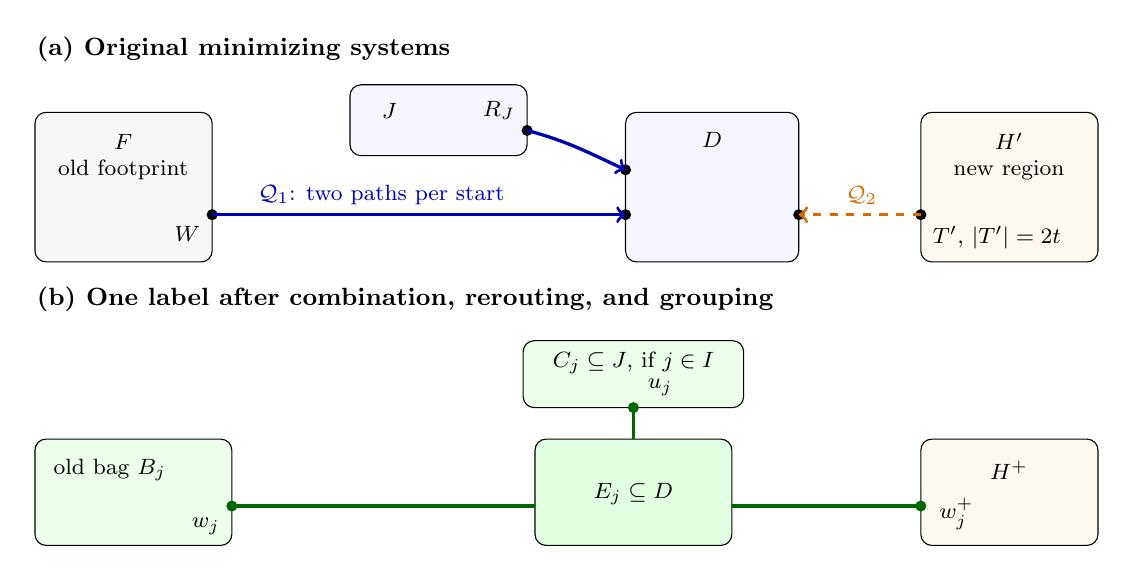
\begin{tikzpicture}[x=1cm,y=1cm,font=\footnotesize]
  \node[anchor=west,font=\small\bfseries] at (0,6.55)
    {(a) Original minimizing systems};
  \draw[rounded corners,fill=black!3] (0.1,3.85) rectangle (2.35,5.75);
  \node at (1.22,5.38) {\(F\)};
  \node at (1.22,5.02) {old footprint};
  \fill (2.35,4.45) circle (2pt);
  \node[below left] at (2.32,4.43) {\(W\)};

  \draw[rounded corners,fill=blue!4] (4.1,5.2) rectangle (6.35,6.1);
  \node at (4.6,5.77) {\(J\)};
  \fill (6.35,5.52) circle (2pt);
  \node[above left] at (6.32,5.53) {\(R_J\)};

  \draw[rounded corners,fill=blue!4] (7.6,3.85) rectangle (9.8,5.75);
  \node at (8.7,5.4) {\(D\)};
  \fill (7.6,4.45) circle (2pt);
  \fill (7.6,5.02) circle (2pt);
  \fill (9.8,4.45) circle (2pt);

  \draw[rounded corners,fill=orange!5] (11.35,3.85) rectangle (13.6,5.75);
  \node at (12.47,5.38) {\(H'\)};
  \node at (12.47,5.02) {new region};
  \fill (11.35,4.45) circle (2pt);
  \node[below right] at (11.38,4.43) {\(T'\), \(|T'|=2t\)};

  \draw[->,very thick,blue!70!black] (2.35,4.45) -- (7.6,4.45);
  \node[above,text=blue!70!black] at (4.5,4.45)
    {\(\mathcal Q_1\): two paths per start};
  \draw[->,very thick,blue!70!black]
    (6.35,5.52) to[out=-15,in=155] (7.6,5.02);
  \draw[->,very thick,dashed,orange!85!black]
    (11.35,4.45) -- (9.8,4.45);
  \node[above,text=orange!85!black] at (10.6,4.45)
    {\(\mathcal Q_2\)};

  \node[anchor=west,font=\small\bfseries] at (0,3.38)
    {(b) One label after combination, rerouting, and grouping};
  \draw[rounded corners,fill=green!8] (0.1,0.25) rectangle (2.6,1.6);
  \node at (1.05,1.21) {old bag \(B_j\)};
  \fill[green!40!black] (2.6,0.75) circle (2pt);
  \node[below left] at (2.57,0.72) {\(w_j\)};

  \draw[rounded corners,fill=green!12] (6.45,0.25) rectangle (8.95,1.6);
  \node at (7.7,0.9) {\(E_j\subseteq D\)};

  \draw[rounded corners,fill=green!8] (6.3,2.0) rectangle (9.1,2.85);
  \node at (7.7,2.57) {\(C_j\subseteq J\), if \(j\in I\)};
  \fill[green!40!black] (7.7,2.0) circle (2pt);
  \node[above right] at (7.76,2.03) {\(u_j\)};
  \draw[very thick,green!40!black] (7.7,2.0) -- (7.7,1.6);

  \draw[rounded corners,fill=orange!5] (11.35,0.25) rectangle (13.6,1.6);
  \node at (12.47,1.21) {\(H^+\)};
  \fill[green!40!black] (11.35,0.75) circle (2pt);
  \node[right] at (11.46,0.65) {\(w_j^+\)};
  \draw[very thick,green!40!black] (2.6,0.75) -- (6.45,0.75);
  \draw[very thick,green!40!black] (8.95,0.75) -- (11.35,0.75);
\end{tikzpicture}
\caption{A separability round, shown schematically.
The upper arrows represent families of paths; the two families may
intersect, and their entire vertex sets remain in the footprint.
Below, \(E_j\) joins label \(j\)'s path ends in \(D\).
The region \(H^+\) is obtained from \(H'\) by removing unused starts;
it meets the footprint exactly in the new tips \(W^+\).}
\label{fig:separability-round}
\end{figure}


Extend \(B_j\) by the two or three corresponding paths, by \(E_j\),
and by \(C_j\) when \(j\in I\). The resulting set \(B_j^+\) is
connected: its old bag contains \(w_j\); the paths join every
attached piece to \(E_j\); and it contains the new tip \(w_j^+\).
The sets \(B_j^+\) are pairwise disjoint. Indeed, the old bags
are disjoint and meet the added paths only at their own \(W\)-ends;
the paths are disjoint; the sets \(E_j\) are disjoint and meet paths
only at the designated terminals; and the bags \(C_j\) are
disjoint, lie outside \(F\cup D\), and meet paths only at their
own roots. All these sets lie in \(F^+\).
Old adjacencies persist because \(B_j\subseteq B_j^+\), and every
pair of labels in \(I\) gains an adjacency through its bags in
the district model.

It remains to check the next-region invariant. Exactly \(t\) vertices
were deleted from the \((K_0+1)t\)-connected
graph \(H'\), so \(H^+\) is \(K_0t\)-connected. By
\eqref{separate:new-region-list} and \eqref{separate:ch},
\[
 \ell(H^+)
 \ge r-\bigl(c_f+6(K_0+1)+1\bigr)t
 \ge r-c_ht.
\]
Equation~\eqref{separate:region-footprint} gives
\[
 V(H^+)\cap F^+=W^+.
\]
Thus \(F^+,H^+,W^+\), and the bags \(B_j^+\) restore every
invariant for the next round.

After all \(R_t\) rounds, every pair of labels has an adjacency.
The \(t\) disjoint connected label bags therefore form a \(K_t\)
model in \(G\), contradicting \(h(G)<t\).
This proves Lemma~\ref{lem:separability}.
\end{proof}
